% =============================================================================
% Lean4-Automata: Technical Architecture Reference
% Documentation Anchor — Commit 10927ba
% =============================================================================
% Compile: pdflatex lean4a_architecture_anchor.tex (run twice for ToC/refs)
% =============================================================================

\documentclass[11pt, a4paper]{article}

% ── Page geometry ────────────────────────────────────────────────────────────
\usepackage[margin=2.5cm]{geometry}

% ── Typography ───────────────────────────────────────────────────────────────
\usepackage[T1]{fontenc}
\usepackage{lmodern}
\usepackage{microtype}

% ── Tables ───────────────────────────────────────────────────────────────────
\usepackage{longtable}
\usepackage{booktabs}
\usepackage{array}

% ── Graphics & Diagrams ─────────────────────────────────────────────────────
\usepackage{tikz}
\usetikzlibrary{arrows.meta, positioning, shapes.geometric}

% ── Code Listings ────────────────────────────────────────────────────────────
\usepackage{listings}
\usepackage{xcolor}

\definecolor{codebg}{HTML}{F8F8F8}
\definecolor{codeframe}{HTML}{CCCCCC}
\definecolor{keyword}{HTML}{0000FF}
\definecolor{string}{HTML}{A31515}
\definecolor{comment}{HTML}{008000}

\lstset{
  basicstyle=\ttfamily\small,
  backgroundcolor=\color{codebg},
  frame=single,
  rulecolor=\color{codeframe},
  keywordstyle=\color{keyword}\bfseries,
  stringstyle=\color{string},
  commentstyle=\color{comment}\itshape,
  showstringspaces=false,
  breaklines=true,
  breakatwhitespace=true,
  tabsize=4,
  captionpos=b,
  numbers=left,
  numberstyle=\tiny\color{gray},
  numbersep=8pt,
  xleftmargin=1.5em,
  aboveskip=1em,
  belowskip=0.8em,
}

% Language definitions
\lstdefinelanguage{Go}{
  morekeywords={package, import, func, var, type, struct, map, chan, interface,
                return, if, else, for, range, switch, case, default, break,
                continue, go, defer, select, const, true, false, nil,
                string, int, int64, bool, error, float64, byte},
  morecomment=[l]{//},
  morecomment=[s]{/*}{*/},
  morestring=[b]",
  morestring=[b]`,
  sensitive=true,
}

\lstdefinelanguage{SQL}{
  morekeywords={CREATE, TABLE, IF, NOT, EXISTS, PRIMARY, KEY, TEXT,
                INTEGER, BOOLEAN, DEFAULT, CHECK, IN, INDEX, ON, DESC,
                TRIGGER, AFTER, INSERT, WHEN, SELECT, COUNT, FROM, WHERE,
                BEGIN, DELETE, ORDER, BY, LIMIT, ASC, AUTOINCREMENT,
                NULL, PRAGMA, END, VIEW, AS, JOIN, LEFT, GROUP, CASE,
                THEN, ELSE},
  morecomment=[l]{--},
  morestring=[b]',
  sensitive=false,
}

% ── Hyperlinks ───────────────────────────────────────────────────────────────
\usepackage[
  colorlinks=true,
  linkcolor=blue!60!black,
  urlcolor=blue!70!black,
  citecolor=green!50!black,
  bookmarks=true,
  bookmarksnumbered=true,
  pdfstartview=FitH,
]{hyperref}

% ── Title info ───────────────────────────────────────────────────────────────
\title{%
  \textbf{Lean4-Automata: Technical Architecture Reference}\\[0.5em]
  \large Documentation Anchor --- Commit \texttt{10927ba}%
}
\author{Auto-generated from codebase survey}
\date{May 2026}

% =============================================================================
\begin{document}

\maketitle
\thispagestyle{empty}

\begin{center}
\small\textit{Source: \texttt{docs/lean4a\_architecture\_anchor\_sections/}
— edit section \texttt{.tex} files and recompile with \texttt{pdflatex} to update.}
\end{center}

\begin{abstract}
This document is the \emph{architecture anchor} for the Lean4-Automata project
at commit \texttt{10927ba} (HEAD of \texttt{main} as of May~2026).  It captures
every database column, HTTP route, environment variable, Go flow-function, and
Docker service so that future checkpoint updates can be expressed as deltas
against this baseline.  The system indexes Lean~4 proof libraries into a
PostgreSQL database, exposes them via dual FastAPI micro-services, and provides
a Go-based forum harness for AI-agent consumption of proof-state intelligence.
\end{abstract}

\tableofcontents
\clearpage

% ── Sections (one file each for incremental maintenance) ─────────────────────

% =============================================================================
% Section 1: Introduction
% =============================================================================

\section{Introduction}
\label{sec:introduction}

\subsection{Purpose}

\textbf{Lean4-Automata} is a full-stack indexing, search, and analysis platform
for Lean~4 proof libraries.  It continuously parses \texttt{.lean} source files,
extracts every top-level declaration (theorems, definitions, axioms, instances,
etc.), computes static-analysis quality signals, and stores the results in a
PostgreSQL database fronted by dual FastAPI micro-services (read-only query API
and admin-only ingestion API).  A Next.js~16 frontend and a Go-based
\emph{forum harness} provide two complementary consumption paths: a rich
browser UI for human analysts and an SSE-driven flow-execution engine for
AI agents (TPH, DynamicFlux, Wolfram) that need machine-readable proof-state
intelligence.

\subsection{Design Goals}

\begin{enumerate}
  \item \textbf{AI-agent consumption.}  Every endpoint returns structured JSON
        with pagination, full-text-search ranking, and dependency-graph
        traversals so that large-language-model agents can reason about proof
        completeness without re-parsing source files.
  \item \textbf{Incremental indexing.}  A file-watcher daemon debounces
        filesystem events, gates on SHA-256 hashes, and upserts only changed
        files—keeping the index fresh with sub-second latency.
  \item \textbf{Static proof-quality signals.}  The parser emits 15+
        \texttt{FileMetrics} fields (\texttt{sorry\_count},
        \texttt{proof\_completion}, \texttt{native\_decide\_count}, etc.)
        that enable proof-health dashboards without elaboration-level tooling.
  \item \textbf{Local-first forum harness.}  The Go forum stores all findings
        in a local SQLite WAL database (\texttt{\textasciitilde/.lean4a/forum.db}),
        ensuring that sensitive proof state never leaves the user's machine
        unless explicitly exported.
  \item \textbf{Observable infrastructure.}  Docker Compose orchestrates
        10~services with health checks, rate limiting, and an optional
        Loki\,+\,Grafana observability stack.
\end{enumerate}

\subsection{Scope of This Document}

This document is the \emph{architecture anchor} at commit
\texttt{10927ba}.  It captures every schema column, every HTTP route, every
environment variable, and the full flow-function registry so that subsequent
checkpoint documents can be expressed as deltas against this baseline.

\clearpage

% =============================================================================
% Section 2: System Overview
% =============================================================================

\section{System Overview}
\label{sec:system-overview}

Figure~\ref{fig:system-layers} shows the six-layer architecture.  Data flows
bottom-to-top: the \emph{Parser} layer watches the filesystem and feeds
PostgreSQL; the \emph{API} layer exposes read/write endpoints; the
\emph{Forum Harness} orchestrates CLI flows via SSE; and the \emph{UI} and
\emph{TPH/Agent} layers consume the results.

\begin{figure}[htbp]
\centering
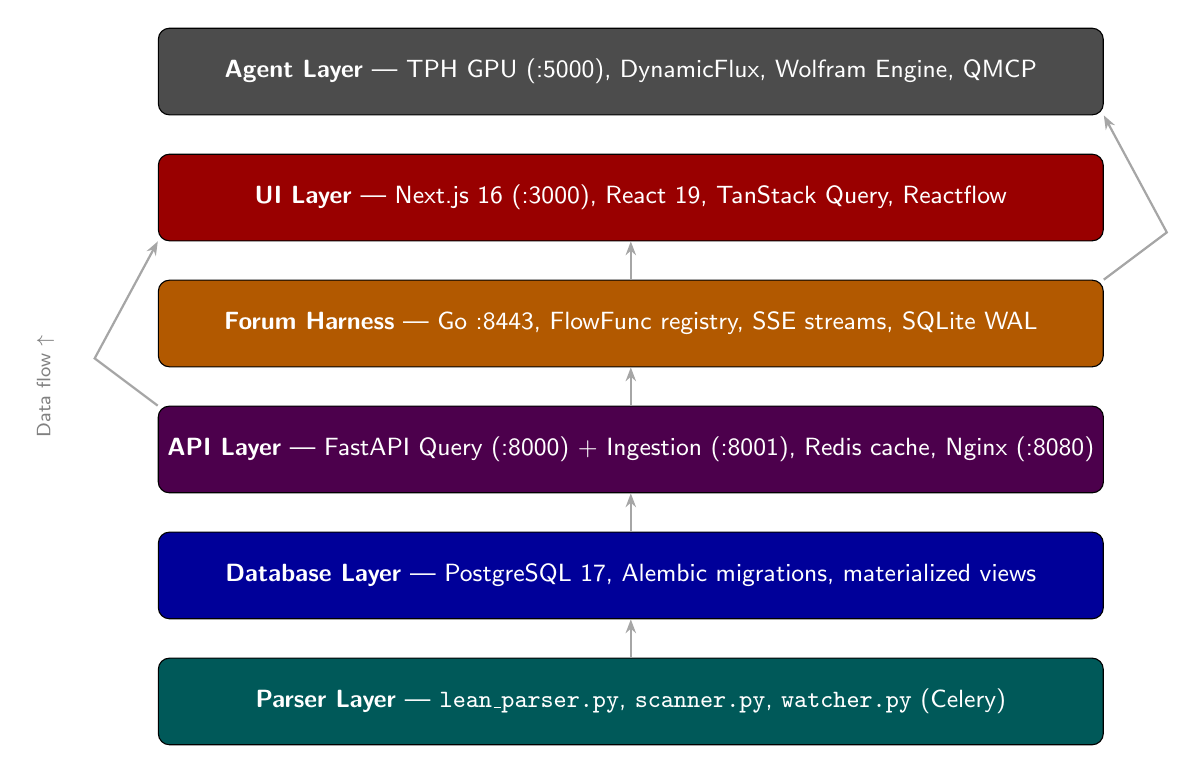
\begin{tikzpicture}[
    layer/.style={
      draw, rounded corners=4pt, minimum width=12cm, minimum height=1.1cm,
      font=\sffamily\small, text=white, align=center
    },
    arrow/.style={-{Stealth[length=5pt]}, thick, gray!70}
  ]

  % Layers (bottom to top)
  \node[layer, fill=teal!70!black]     (parser) at (0,0)
    {\textbf{Parser Layer} — \texttt{lean\_parser.py}, \texttt{scanner.py}, \texttt{watcher.py} (Celery)};
  \node[layer, fill=blue!60!black]     (db)     at (0,1.6)
    {\textbf{Database Layer} — PostgreSQL 17, Alembic migrations, materialized views};
  \node[layer, fill=violet!60!black]   (api)    at (0,3.2)
    {\textbf{API Layer} — FastAPI Query (:8000) + Ingestion (:8001), Redis cache, Nginx (:8080)};
  \node[layer, fill=orange!70!black]   (forum)  at (0,4.8)
    {\textbf{Forum Harness} — Go :8443, FlowFunc registry, SSE streams, SQLite WAL};
  \node[layer, fill=red!60!black]      (ui)     at (0,6.4)
    {\textbf{UI Layer} — Next.js 16 (:3000), React 19, TanStack Query, Reactflow};
  \node[layer, fill=gray!60!black]     (agent)  at (0,8.0)
    {\textbf{Agent Layer} — TPH GPU (:5000), DynamicFlux, Wolfram Engine, QMCP};

  % Arrows
  \draw[arrow] (parser.north) -- (db.south);
  \draw[arrow] (db.north)     -- (api.south);
  \draw[arrow] (api.north)    -- (forum.south);
  \draw[arrow] (forum.north)  -- (ui.south);
  \draw[arrow] (forum.north east) -- ++(0.8,0.6) -- (agent.south east);
  \draw[arrow] (api.north west)   -- ++(-0.8,0.6) -- (ui.south west);

  % Side annotations
  \node[font=\scriptsize\sffamily, gray, rotate=90, anchor=south] at (-7.2,4.0)
    {Data flow $\uparrow$};

\end{tikzpicture}
\caption{Six-layer architecture of Lean4-Automata at commit \texttt{10927ba}.}
\label{fig:system-layers}
\end{figure}

\subsection{Key Technology Choices}

\begin{tabular}{@{}lll@{}}
\toprule
\textbf{Layer}       & \textbf{Technology}            & \textbf{Rationale} \\
\midrule
Parser               & Python 3.11, regex-based       & Fast; no Lean toolchain dependency \\
Database             & PostgreSQL 17, JSONB, GIN      & Rich indexing, CTE support \\
Cache                & Redis 7, pub/sub               & Cache-aside + invalidation bus \\
Query API            & FastAPI + Uvicorn              & Async, OpenAPI, SSE native \\
Ingestion API        & FastAPI + Celery               & Async task queue for long scans \\
Forum Harness        & Go 1.21+, SQLite WAL           & Low-latency subprocess control \\
Frontend             & Next.js 16, React 19           & App Router, SSR, TanStack Query \\
Observability        & Loki 3.4 + Grafana 11.6        & Structured log aggregation \\
\bottomrule
\end{tabular}

\clearpage

% =============================================================================
% Section 3: Database Schema
% =============================================================================

\section{Database Schema}
\label{sec:database-schema}

The PostgreSQL schema is managed by Alembic (async driver \texttt{asyncpg}).
The migration chain is:

\begin{center}
\begin{tabular}{@{}clll@{}}
\toprule
\textbf{Rev} & \textbf{File} & \textbf{Description} & \textbf{Objects Created} \\
\midrule
0001 & \texttt{0001\_initial\_schema.py} & Core tables + enums & 6 tables, 2 enums \\
0002 & \texttt{0002\_add\_indexes.py}    & B-tree + GIN indexes & 20+ indexes \\
0003 & \texttt{0003\_materialized\_views.py} & Centrality + module metrics & 2 mat.\ views \\
0004 & \texttt{0004\_enriched\_metrics.py}  & Phase~2 static-analysis & 15 columns, 3 views \\
\bottomrule
\end{tabular}
\end{center}

% ── projects ─────────────────────────────────────────────────────────────────
\subsection{Table: \texttt{projects}}

\begin{longtable}{@{}llp{6.5cm}@{}}
\toprule
\textbf{Column} & \textbf{Type} & \textbf{Notes} \\
\midrule
\endfirsthead
\toprule
\textbf{Column} & \textbf{Type} & \textbf{Notes} \\
\midrule
\endhead
\bottomrule
\endfoot
id              & \texttt{INTEGER} PK  & Auto-increment \\
name            & \texttt{VARCHAR(255)} & \texttt{NOT NULL, UNIQUE} \\
root\_path      & \texttt{TEXT}         & Filesystem root \\
lean\_version   & \texttt{VARCHAR(50)}  & e.g.\ \texttt{"4.8.0"} \\
lakefile\_hash  & \texttt{VARCHAR(64)}  & Lake config hash \\
indexed\_at     & \texttt{TIMESTAMPTZ}  & Default \texttt{now()} \\
last\_modified  & \texttt{TIMESTAMPTZ}  & Default \texttt{now()} \\
metadata        & \texttt{JSONB}        & Free-form metadata \\
\end{longtable}

% ── files ────────────────────────────────────────────────────────────────────
\subsection{Table: \texttt{files}}
\label{subsec:files-table}

\begin{longtable}{@{}llp{6cm}@{}}
\toprule
\textbf{Column} & \textbf{Type} & \textbf{Notes} \\
\midrule
\endfirsthead
\toprule
\textbf{Column} & \textbf{Type} & \textbf{Notes} \\
\midrule
\endhead
\bottomrule
\endfoot
id                      & \texttt{INTEGER} PK       & Auto-increment \\
project\_id             & \texttt{INTEGER} FK       & \texttt{projects.id}, CASCADE \\
relative\_path          & \texttt{TEXT}              & Path relative to project root \\
absolute\_path          & \texttt{TEXT}              & Full filesystem path \\
module\_name            & \texttt{TEXT}              & Lean module name \\
file\_hash              & \texttt{VARCHAR(64)}       & SHA-256 (hash gate) \\
line\_count             & \texttt{INTEGER}           & Number of lines \\
char\_count             & \texttt{INTEGER}           & Number of characters \\
indexed\_at             & \texttt{TIMESTAMPTZ}       & Default \texttt{now()} \\
last\_modified          & \texttt{TIMESTAMPTZ}       & Default \texttt{now()} \\
imports                 & \texttt{JSONB}             & JSON array of import strings \\
metadata                & \texttt{JSONB}             & Free-form metadata \\
\midrule
\multicolumn{3}{@{}l}{\textit{Phase~2 enriched columns (migration 0004):}} \\
\midrule
sorry\_count            & \texttt{INTEGER}           & Default 0. Raw \texttt{sorry} occurrences \\
admit\_count            & \texttt{INTEGER}           & Default 0. Raw \texttt{admit} occurrences \\
sorry\_lines            & \texttt{JSONB}             & Default \texttt{[]}. 1-based line numbers \\
sorry\_in\_proof\_count & \texttt{INTEGER}           & Default 0. Theorems with sorry in body \\
theorem\_count          & \texttt{INTEGER}           & Default 0. Total theorems + lemmas \\
proof\_completion       & \texttt{FLOAT}             & Default 1.0. Ratio of complete proofs \\
native\_decide\_count   & \texttt{INTEGER}           & Default 0. Fragile kernel decisions \\
debug\_command\_count   & \texttt{INTEGER}           & Default 0. Leftover \texttt{\#check}/\texttt{\#eval} \\
noncomputable\_count    & \texttt{INTEGER}           & Default 0. \texttt{noncomputable} decls \\
instance\_count         & \texttt{INTEGER}           & Default 0. Typeclass instances \\
declared\_axiom\_count  & \texttt{INTEGER}           & Default 0. Custom axiom decls \\
simp\_attr\_count       & \texttt{INTEGER}           & Default 0. \texttt{@[simp]} tagged lemmas \\
docstring\_count        & \texttt{INTEGER}           & Default 0. Doc comments present \\
todo\_count             & \texttt{INTEGER}           & Default 0. TODO/FIXME/HACK/XXX \\
mathlib\_import\_count  & \texttt{INTEGER}           & Default 0. Imports from \texttt{Mathlib.*} \\
\end{longtable}

\noindent\textbf{Unique constraint:} \texttt{(project\_id, relative\_path)}.

% ── symbols ──────────────────────────────────────────────────────────────────
\subsection{Table: \texttt{symbols}}

\begin{longtable}{@{}llp{6cm}@{}}
\toprule
\textbf{Column} & \textbf{Type} & \textbf{Notes} \\
\midrule
\endfirsthead
\toprule
\textbf{Column} & \textbf{Type} & \textbf{Notes} \\
\midrule
\endhead
\bottomrule
\endfoot
id              & \texttt{INTEGER} PK     & Auto-increment \\
file\_id        & \texttt{INTEGER} FK     & \texttt{files.id}, CASCADE \\
project\_id     & \texttt{INTEGER} FK     & \texttt{projects.id}, CASCADE \\
name            & \texttt{TEXT}            & Short name (\texttt{"append"}) \\
full\_name      & \texttt{TEXT}            & Qualified name (\texttt{"List.append"}) \\
kind            & \texttt{symbol\_kind}    & Enum (see below) \\
line\_start     & \texttt{INTEGER}         & 1-based start line \\
line\_end       & \texttt{INTEGER}         & Inclusive end line \\
col\_start      & \texttt{INTEGER}         & 1-based column start \\
col\_end        & \texttt{INTEGER}         & 1-based column end \\
signature       & \texttt{TEXT}            & Lean signature text \\
docstring       & \texttt{TEXT}            & \texttt{/-- ... -/} doc comment \\
is\_public      & \texttt{BOOLEAN}         & Default \texttt{true} \\
is\_deprecated  & \texttt{BOOLEAN}         & Default \texttt{false} \\
indexed\_at     & \texttt{TIMESTAMPTZ}     & Default \texttt{now()} \\
attributes      & \texttt{JSONB}           & e.g.\ \texttt{["@[simp]"]} \\
metadata        & \texttt{JSONB}           & Free-form \\
has\_sorry      & \texttt{BOOLEAN}         & Default \texttt{false} (Phase~2) \\
\end{longtable}

\noindent\textbf{Unique constraint:} \texttt{(project\_id, full\_name)}.

\noindent\textbf{\texttt{symbol\_kind} enum values:}
\texttt{theorem}, \texttt{def}, \texttt{axiom}, \texttt{instance},
\texttt{inductive}, \texttt{structure}, \texttt{class}, \texttt{constant},
\texttt{opaque}, \texttt{abbrev}.

% ── dependencies ─────────────────────────────────────────────────────────────
\subsection{Table: \texttt{dependencies}}

\begin{longtable}{@{}llp{6cm}@{}}
\toprule
\textbf{Column} & \textbf{Type} & \textbf{Notes} \\
\midrule
\endfirsthead
\bottomrule
\endfoot
id                  & \texttt{INTEGER} PK  & Auto-increment \\
source\_symbol\_id  & \texttt{INTEGER} FK  & \texttt{symbols.id}, CASCADE \\
target\_symbol\_id  & \texttt{INTEGER} FK  & \texttt{symbols.id}, CASCADE \\
dependency\_type    & \texttt{dep\_type}    & Enum: \texttt{direct}, \texttt{implicit}, \texttt{import}, \texttt{indirect} \\
confidence          & \texttt{FLOAT}        & Default 1.0 (0.0--1.0) \\
indexed\_at         & \texttt{TIMESTAMPTZ}  & Default \texttt{now()} \\
provenance          & \texttt{TEXT}         & Detection method \\
metadata            & \texttt{JSONB}        & Free-form \\
\end{longtable}

% ── file_dependencies ────────────────────────────────────────────────────────
\subsection{Table: \texttt{file\_dependencies}}

\begin{longtable}{@{}llp{6cm}@{}}
\toprule
\textbf{Column} & \textbf{Type} & \textbf{Notes} \\
\midrule
\endfirsthead
\bottomrule
\endfoot
id                & \texttt{INTEGER} PK  & Auto-increment \\
source\_file\_id  & \texttt{INTEGER} FK  & \texttt{files.id}, CASCADE \\
target\_file\_id  & \texttt{INTEGER} FK  & \texttt{files.id}, CASCADE \\
is\_direct\_import& \texttt{BOOLEAN}     & Default \texttt{true} \\
indexed\_at       & \texttt{TIMESTAMPTZ} & Default \texttt{now()} \\
\end{longtable}

% ── index_runs ───────────────────────────────────────────────────────────────
\subsection{Table: \texttt{index\_runs}}

\begin{longtable}{@{}llp{6cm}@{}}
\toprule
\textbf{Column} & \textbf{Type} & \textbf{Notes} \\
\midrule
\endfirsthead
\bottomrule
\endfoot
id                & \texttt{INTEGER} PK    & Auto-increment \\
project\_id       & \texttt{INTEGER} FK    & \texttt{projects.id}, CASCADE \\
run\_type         & \texttt{VARCHAR(50)}    & \texttt{"full\_scan"} or \texttt{"incremental"} \\
started\_at       & \texttt{TIMESTAMPTZ}    & Default \texttt{now()} \\
completed\_at     & \texttt{TIMESTAMPTZ}    & Nullable \\
files\_processed  & \texttt{INTEGER}        & Default 0 \\
symbols\_indexed  & \texttt{INTEGER}        & Default 0 \\
errors            & \texttt{JSONB}          & Default \texttt{[]} \\
status            & \texttt{VARCHAR(50)}    & \texttt{"running"}, \texttt{"success"}, \texttt{"failed"} \\
\end{longtable}

% ── Views ────────────────────────────────────────────────────────────────────
\subsection{Views (Migration 0004)}

\paragraph{\texttt{v\_proof\_status}} Per-file proof completeness.
Key columns: \texttt{relative\_path}, \texttt{theorem\_count},
\texttt{sorry\_in\_proof\_count}, \texttt{proof\_completion},
\texttt{proof\_status} (derived: \texttt{complete}, \texttt{partial},
\texttt{mostly\_incomplete}, \texttt{no\_theorems}).

\paragraph{\texttt{v\_floating\_symbols}} Public theorems/defs with zero
incoming cross-file dependencies---proved but never referenced.

\paragraph{\texttt{v\_file\_interconnect}} File-level fan-in/fan-out,
\texttt{mathlib\_import\_count}, \texttt{local\_import\_count}, and per-file
health summary.

\subsection{Materialized Views (Migration 0003)}

\paragraph{\texttt{dependency\_stats}} Per-symbol centrality:
\texttt{outgoing\_dependencies}, \texttt{incoming\_dependencies},
\texttt{total\_connections}, \texttt{fan\_out\_ratio}.

\paragraph{\texttt{module\_metrics}} Per-module aggregations: symbol counts by
kind, \texttt{avg\_symbol\_length\_lines}, \texttt{documentation\_coverage\_pct}.

\clearpage

% =============================================================================
% Section 4: Parser Static-Analysis Signals
% =============================================================================

\section{Parser Static-Analysis Signals}
\label{sec:parser-signals}

The regex-based parser (\texttt{parser/lean\_parser.py}) extracts top-level
declarations without requiring a Lean~4 elaborator.  For each \texttt{.lean}
file it produces a \texttt{FileMetrics} frozen dataclass whose fields map 1:1
to columns on the \texttt{files} table (added in migration 0004).

\subsection{\texttt{FileMetrics} Fields}

\begin{longtable}{@{}llp{4.8cm}l@{}}
\toprule
\textbf{Field} & \textbf{Type} & \textbf{Description} & \textbf{SQL Column} \\
\midrule
\endfirsthead
\toprule
\textbf{Field} & \textbf{Type} & \textbf{Description} & \textbf{SQL Column} \\
\midrule
\endhead
\bottomrule
\endfoot
\multicolumn{4}{@{}l}{\textit{Proof completeness}} \\
\midrule
sorry\_count          & \texttt{int}        & Raw \texttt{sorry} occurrences        & \texttt{sorry\_count} \\
admit\_count          & \texttt{int}        & Raw \texttt{admit} occurrences        & \texttt{admit\_count} \\
sorry\_lines          & \texttt{list[int]}  & 1-based line numbers of sorrys        & \texttt{sorry\_lines} \\
sorry\_in\_proof\_count & \texttt{int}      & Theorems whose body contains sorry    & \texttt{sorry\_in\_proof\_count} \\
theorem\_count        & \texttt{int}        & Total theorems + lemmas               & \texttt{theorem\_count} \\
proof\_completion     & \texttt{float}      & $\frac{\text{thm\_count} - \text{sorry\_in\_proof}}{\text{thm\_count}}$ & \texttt{proof\_completion} \\
\midrule
\multicolumn{4}{@{}l}{\textit{Fragility signals}} \\
\midrule
native\_decide\_count & \texttt{int}        & \texttt{native\_decide} (kernel-level, fragile) & \texttt{native\_decide\_count} \\
debug\_command\_count & \texttt{int}        & Leftover \texttt{\#check}/\texttt{\#eval}/\texttt{\#print} & \texttt{debug\_command\_count} \\
\midrule
\multicolumn{4}{@{}l}{\textit{Symbol counts}} \\
\midrule
noncomputable\_count  & \texttt{int}        & \texttt{noncomputable} declarations   & \texttt{noncomputable\_count} \\
instance\_count       & \texttt{int}        & Typeclass instances                   & \texttt{instance\_count} \\
declared\_axiom\_count& \texttt{int}        & Custom \texttt{axiom} declarations    & \texttt{declared\_axiom\_count} \\
simp\_attr\_count     & \texttt{int}        & \texttt{@[simp]}-tagged lemmas        & \texttt{simp\_attr\_count} \\
\midrule
\multicolumn{4}{@{}l}{\textit{Documentation / hygiene}} \\
\midrule
docstring\_count      & \texttt{int}        & \texttt{/-- ... -/} docstrings        & \texttt{docstring\_count} \\
todo\_count           & \texttt{int}        & TODO / FIXME / HACK / XXX comments    & \texttt{todo\_count} \\
\midrule
\multicolumn{4}{@{}l}{\textit{Import profile}} \\
\midrule
mathlib\_import\_count& \texttt{int}        & Imports from \texttt{Mathlib.*}       & \texttt{mathlib\_import\_count} \\
\end{longtable}

\subsection{\texttt{ParsedSymbol} Fields}

Each top-level Lean declaration yields a \texttt{ParsedSymbol}:

\begin{longtable}{@{}llp{6cm}@{}}
\toprule
\textbf{Field} & \textbf{Type} & \textbf{Description} \\
\midrule
\endfirsthead
\bottomrule
\endfoot
name             & \texttt{str}  & Short name (e.g.\ \texttt{"append"}) \\
kind             & \texttt{str}  & Kind keyword (\texttt{def}, \texttt{theorem}, \texttt{lemma}, \ldots) \\
line\_start      & \texttt{int}  & 1-based line number \\
namespace\_path  & \texttt{str}  & Namespace context (e.g.\ \texttt{"List"}) \\
is\_private      & \texttt{bool} & Whether marked \texttt{private} \\
signature\_text  & \texttt{str}  & Lean signature snippet \\
mods             & \texttt{str}  & Raw modifier string (e.g.\ \texttt{"@[simp] noncomputable"}) \\
has\_sorry       & \texttt{bool} & \texttt{sorry}/\texttt{admit} found in declaration body \\
\end{longtable}

\noindent\textbf{Kind mapping:}
The parser recognises 11~keywords (\texttt{def}, \texttt{theorem},
\texttt{lemma}, \texttt{instance}, \texttt{class}, \texttt{structure},
\texttt{inductive}, \texttt{abbrev}, \texttt{axiom}, \texttt{example},
\texttt{opaque}).  At the DB layer \texttt{lemma}~$\to$~\texttt{theorem}
(collapsed) and \texttt{example} is dropped.

\subsection{Parse Pipeline}

\begin{enumerate}
  \item Strip single-line (\texttt{-{}-}) and block (\texttt{/- \ldots -/})
        comments, preserving line numbers.
  \item Extract imports: \lstinline[language=Python]{r"^\s*import\s+([A-Za-z0-9_.]+)\s*$"}
  \item Track \texttt{namespace}/\texttt{end} blocks for fully-qualified names.
  \item Match declaration heads via modifier\,+\,kind\,+\,name regex.
  \item Scan for \texttt{sorry}, \texttt{admit}, \texttt{native\_decide},
        \texttt{\#check}, \texttt{\#eval}, \texttt{@[simp]}, etc.
  \item Aggregate into \texttt{FileMetrics}.
\end{enumerate}

\noindent\textbf{Constraint:} Not a full Lean~4 grammar---regex extraction of
declaration \emph{heads} only; tactic blocks and elaborator macros are out of
scope.

\clearpage

% =============================================================================
% Section 5: Python API Routes
% =============================================================================

\section{Python API Routes}
\label{sec:api-routes}

Two FastAPI applications expose the database to consumers.

\subsection{Query API (\texttt{:8000})}

Base prefix: \texttt{/api/v1}.  CORS allowed from \texttt{http://localhost:3000}.
No authentication required.

\begin{longtable}{@{}llp{5.5cm}@{}}
\toprule
\textbf{Method / Path} & \textbf{Handler} & \textbf{Description} \\
\midrule
\endfirsthead
\toprule
\textbf{Method / Path} & \textbf{Handler} & \textbf{Description} \\
\midrule
\endhead
\bottomrule
\endfoot
\texttt{GET /health/live}
  & liveness & Returns \texttt{\{"status":"alive"\}} \\
\texttt{GET /health/ready}
  & readiness & Checks DB + Redis; returns booleans \\
\texttt{GET /api/v1/symbols/search}
  & \texttt{search\_symbols} & Full-text search.  Params: \texttt{q}, \texttt{project\_id}, \texttt{limit} (1--100), \texttt{offset} \\
\texttt{GET /api/v1/symbols/\{full\_name\}}
  & \texttt{get\_symbol} & Lookup by qualified name \\
\texttt{GET /api/v1/dependencies/graph}
  & \texttt{get\_dep\_graph} & Transitive + reverse deps.  Params: \texttt{full\_name}, \texttt{max\_depth} (1--20) \\
\texttt{GET /api/v1/modules/metrics}
  & \texttt{get\_module\_metrics} & Module-level aggregations.  Params: \texttt{project\_id}, \texttt{order\_by} \\
\texttt{GET /api/v1/events/invalidation}
  & SSE stream & \texttt{text/event-stream}; publishes cache-invalidation events \\
\end{longtable}

\paragraph{Cache strategy.}
Redis cache-aside with 1-hour TTL.  Keys follow the pattern
\texttt{lean4:cache:\{entity\}:\{params\}}.  Invalidation is broadcast via
Redis pub/sub channel \texttt{lean4:invalidate}.

\subsection{Ingestion API (\texttt{:8001})}

Base prefix: \texttt{/admin}.  Requires Bearer JWT with \texttt{role:"admin"}.

\begin{longtable}{@{}llp{5.5cm}@{}}
\toprule
\textbf{Method / Path} & \textbf{Handler} & \textbf{Description} \\
\midrule
\endfirsthead
\bottomrule
\endfoot
\texttt{POST /health/live}
  & liveness & Returns \texttt{\{"status":"alive"\}} \\
\texttt{POST /health/ready}
  & readiness & DB + Redis check (503 if unhealthy) \\
\texttt{POST /admin/index/start}
  & \texttt{start\_index} & Enqueue Celery full-scan.  Body: \texttt{project\_id}, \texttt{root\_dir}.  Returns 202 with \texttt{task\_id} \\
\texttt{GET /admin/index/status/\{task\_id\}}
  & \texttt{index\_status} & Poll Celery task state \\
\end{longtable}

\subsection{Celery Workers}

\begin{longtable}{@{}lp{7cm}@{}}
\toprule
\textbf{Task} & \textbf{Description} \\
\midrule
\endfirsthead
\bottomrule
\endfoot
\texttt{full\_scan\_task}
  & Parse all \texttt{.lean} files under \texttt{root\_dir}, upsert to DB \\
\texttt{refresh\_views\_task}
  & Refresh materialized views (\texttt{dependency\_stats}, \texttt{module\_metrics}).  Scheduled via Celery Beat \\
\end{longtable}

\clearpage

% =============================================================================
% Section 6: Go Forum Harness
% =============================================================================

\section{Go Forum Harness}
\label{sec:forum-harness}

The forum harness is a Go HTTP server (\texttt{go/forum.go}, port~8443) that
extends the existing Go\_Red QMCP consent gate with a flow-execution engine,
SSE log streaming, ticket storage, and proxy endpoints for the Lean4-Automata
and TPH APIs.

\subsection{HTTP Routes}

\begin{longtable}{@{}llp{5cm}@{}}
\toprule
\textbf{Method / Path} & \textbf{Handler} & \textbf{Description} \\
\midrule
\endfirsthead
\toprule
\textbf{Method / Path} & \textbf{Handler} & \textbf{Description} \\
\midrule
\endhead
\bottomrule
\endfoot
\texttt{GET  /flows}              & \texttt{handleListFlows}    & List all flow definitions \\
\texttt{POST /flows/\{name\}/start} & \texttt{handleStartFlow}  & Execute a named flow \\
\texttt{GET  /flows/\{name\}/events}& SSE stream                & Real-time execution logs \\
\texttt{GET  /tickets/\{id\}}     & \texttt{handleGetTicket}    & Retrieve ticket by ID \\
\texttt{GET  /tickets}            & \texttt{handleListTickets}  & List recent tickets (paginated) \\
\texttt{POST /sessions}           & \texttt{handleCreateSession}& Create a new session \\
\texttt{GET  /sessions}           & \texttt{handleListSessions} & List sessions \\
\texttt{GET  /sessions/\{id\}}    & \texttt{handleGetSession}   & Session details + tickets \\
\texttt{POST /lean/query}         & proxy                       & Forward to Lean4-Automata query API \\
\texttt{POST /tph/inference}      & proxy                       & Forward to TPH GPU server \\
\texttt{GET  /env/status}         & \texttt{handleEnvStatus}    & Python env + GPU check \\
\texttt{GET  /health}             & health                      & DB + upstream health \\
\end{longtable}

\subsection{\texttt{FlowFunc} Registry}

All flows are compiled into the binary---no runtime code execution.  The
\texttt{CommandTemplate} field (present in early designs) was eliminated in
commit \texttt{10927ba}.

\begin{lstlisting}[language=Go, caption={FlowFunc type signature}]
type FlowFunc func(
    ctx     context.Context,
    params  map[string]interface{},
    w       http.ResponseWriter,
    flusher http.Flusher,
) (json.RawMessage, string, string)
\end{lstlisting}

\begin{longtable}{@{}lllp{3.2cm}@{}}
\toprule
\textbf{Flow Name} & \textbf{Handler} & \textbf{Type} & \textbf{Endpoint / Notes} \\
\midrule
\endfirsthead
\toprule
\textbf{Flow Name} & \textbf{Handler} & \textbf{Type} & \textbf{Endpoint / Notes} \\
\midrule
\endhead
\bottomrule
\endfoot
\texttt{lean\_sorry\_scan}        & \texttt{flowLeanSorryScan}        & builtin & \texttt{/api/v1/} query \\
\texttt{lean\_float\_scan}        & \texttt{flowLeanFloatScan}        & builtin & \texttt{v\_floating\_symbols} \\
\texttt{lean\_file\_interconnect} & \texttt{flowLeanFileInterconnect} & builtin & \texttt{v\_file\_interconnect} \\
\texttt{lean\_db\_health}         & \texttt{flowLeanDBHealth}         & builtin & DB stats query \\
\texttt{quick\_proof\_report}     & \texttt{flowQuickProofReport}     & builtin & Composite report \\
\texttt{tph\_inference}           & \texttt{flowTPHInference}         & proxy   & \texttt{:5000/inference} \\
\texttt{tph\_status}              & \texttt{flowTPHStatus}            & proxy   & \texttt{:5000/status} \\
\texttt{env\_check}               & \texttt{flowEnvCheck}             & builtin & Python env probe \\
\texttt{gpu\_check}               & \texttt{flowGPUCheck}             & builtin & ROCm / AMD GPU \\
\texttt{formula\_match}           & placeholder                      & ---     & \emph{Not implemented} \\
\texttt{wolfram\_verify}          & placeholder                      & ---     & \emph{Not implemented} \\
\texttt{lean\_diff\_mathlib}      & placeholder                      & ---     & \emph{Not implemented} \\
\end{longtable}

\subsection{SQLite Forum Schema}

\textbf{Path:} \texttt{\textasciitilde/.lean4a/forum.db} (WAL mode).
Four tables:

\begin{description}
  \item[\texttt{tickets}] (\texttt{id TEXT PK}):
    Flow results.  Columns: \texttt{flow\_name}, \texttt{input\_json},
    \texttt{output\_json}, \texttt{status}
    (\texttt{CHECK IN ('success','error','timeout')}),
    \texttt{error\_message}, \texttt{created\_at} (unix), \texttt{duration\_ms},
    \texttt{tags} (JSON array).
  \item[\texttt{sessions}] (\texttt{id TEXT PK}):
    Ticket groups.  Columns: \texttt{name}, \texttt{created\_at},
    \texttt{ticket\_ids\_json}.
  \item[\texttt{flow\_definitions}] (\texttt{name TEXT PK}):
    Flow metadata.  Columns: \texttt{description}, \texttt{params\_schema}
    (JSON schema), \texttt{handler\_type} (\texttt{builtin}/\texttt{proxy}),
    \texttt{target\_url}, \texttt{enabled}, \texttt{tags}.
  \item[\texttt{flow\_logs}] (\texttt{id INTEGER PK AUTOINCREMENT}):
    Circular buffer (trigger caps at 1000~rows).  Columns: \texttt{flow\_name},
    \texttt{ticket\_id}, \texttt{level}, \texttt{message}, \texttt{timestamp}.
\end{description}

\subsection{Security Posture}

\begin{enumerate}
  \item \textbf{No \texttt{CommandTemplate}.}  Commit \texttt{10927ba}
        eliminated the \texttt{command\_template} field.  All flows are
        compile-time Go functions---no runtime string interpolation into
        shell commands.
  \item \textbf{Method enforcement.}  The router checks HTTP method per
        endpoint (e.g.\ \texttt{POST} only for \texttt{/flows/\{name\}/start}).
  \item \textbf{XSS mitigations.}  The single-file HTML UI
        (\texttt{lean4a\_forum.html}) escapes all dynamic content rendered into
        the DOM.  JSON payloads are displayed via \texttt{<pre>} with
        entity-escaped text.
  \item \textbf{Rate limiting.}  Flow semaphore caps concurrent executions at
        \texttt{MAX\_CONCURRENT\_FLOWS} (default~5).  SSE connections time out
        after 5~minutes.
  \item \textbf{Local-first privacy.}  SQLite lives on the user's filesystem;
        no data leaves the machine unless the user explicitly exports.
\end{enumerate}

\clearpage

% =============================================================================
% Section 7: Infrastructure Services
% =============================================================================

\section{Infrastructure Services}
\label{sec:infrastructure}

All services are orchestrated via \texttt{docker-compose.yml} (217~lines).
The observability stack (Loki + Grafana) is gated behind a Docker Compose
\texttt{profile}.

\subsection{Service Matrix}

\begin{longtable}{@{}lllll@{}}
\toprule
\textbf{Service} & \textbf{Image} & \textbf{Port} & \textbf{Health Check} & \textbf{Depends On} \\
\midrule
\endfirsthead
\toprule
\textbf{Service} & \textbf{Image} & \textbf{Port} & \textbf{Health Check} & \textbf{Depends On} \\
\midrule
\endhead
\bottomrule
\endfoot
postgres        & \texttt{postgres:17}             & 5432 & \texttt{pg\_isready}   & --- \\
redis           & \texttt{redis:7}                 & 6379 & \texttt{redis-cli ping}& --- \\
nginx           & \texttt{nginx:stable}            & 8080 & \texttt{nginx -t}      & app, app\_ingestion \\
app             & \texttt{Dockerfile.api}          & 8000 & \texttt{curl /health/ready} & postgres, redis \\
app\_ingestion  & \texttt{Dockerfile.ingestion}    & 8001 & \texttt{curl /health/ready} & postgres, redis \\
worker          & \texttt{Dockerfile.worker}       & ---  & ---                    & postgres, redis \\
watcher         & \texttt{Dockerfile.worker}       & ---  & ---                    & postgres, redis \\
flower          & \texttt{mher/flower:2.0}         & 5555 & ---                    & redis \\
web             & \texttt{frontend/Dockerfile}     & 3000 & \texttt{wget :3000/}   & nginx \\
loki\textsuperscript{$\dagger$}
                & \texttt{grafana/loki:3.4.2}      & 3100 & \texttt{wget /ready}   & --- \\
grafana\textsuperscript{$\dagger$}
                & \texttt{grafana/grafana:11.6.0}  & 3001 & \texttt{wget /api/health} & loki \\
\end{longtable}

\noindent\textsuperscript{$\dagger$}\,Observability profile only
(\texttt{docker compose -{}-profile observability up}).

\subsection{Nginx Reverse Proxy}

\textbf{Config:} \texttt{nginx/nginx.conf} (121~lines).\\
\textbf{Workers:} \texttt{auto} (CPU count), 2048~connections.

\paragraph{Rate limiting zones.}
\begin{lstlisting}[language=bash, caption={Nginx rate-limit zones}]
limit_conn_zone $binary_remote_addr zone=sse_conn:10m;
limit_req_zone  $binary_remote_addr zone=search_req:10m rate=60r/m;
\end{lstlisting}

\paragraph{Location routing.}

\begin{longtable}{@{}llll@{}}
\toprule
\textbf{Location} & \textbf{Upstream} & \textbf{Rate Limit} & \textbf{Notes} \\
\midrule
\endfirsthead
\bottomrule
\endfoot
\texttt{/api/v1/events/}     & \texttt{app:8000}            & 10 conn/IP    & SSE: buffering off, 1h timeout \\
\texttt{/api/v1/symbols/search} & \texttt{app:8000}         & 60 req/min +20 burst & Search endpoint \\
\texttt{/admin/}              & \texttt{app\_ingestion:8001} & ---           & Path rewrite \\
\texttt{/} (default)          & \texttt{app:8000}            & ---           & All other routes \\
\end{longtable}

\subsection{Volumes}

\begin{tabular}{@{}ll@{}}
\toprule
\textbf{Volume} & \textbf{Mount Point} \\
\midrule
\texttt{postgres\_data}  & \texttt{/var/lib/postgresql/data} \\
\texttt{redis\_data}     & \texttt{/data} (AOF persistence) \\
\texttt{loki\_data}      & \texttt{/loki} \\
\texttt{grafana\_data}   & \texttt{/var/lib/grafana} \\
\texttt{LEAN\_WATCH\_ROOT} & \texttt{/lean-src:ro} (bind mount) \\
\bottomrule
\end{tabular}

\clearpage

% =============================================================================
% Section 8: Configuration Reference
% =============================================================================

\section{Configuration Reference}
\label{sec:configuration}

All configuration is via environment variables, sourced from \texttt{.env}
(template: \texttt{.env.example}, 38~lines).

\subsection{Application \& Ports}

\begin{longtable}{@{}llp{5.5cm}@{}}
\toprule
\textbf{Variable} & \textbf{Default} & \textbf{Description} \\
\midrule
\endfirsthead
\bottomrule
\endfoot
\texttt{APP\_PORT}         & 8000  & Query API listen port \\
\texttt{INGESTION\_PORT}   & 8001  & Ingestion API listen port \\
\texttt{NGINX\_HTTP\_PORT} & 8080  & Nginx reverse proxy port \\
\texttt{FRONTEND\_PORT}    & 3000  & Next.js frontend port \\
\texttt{FLOWER\_PORT}      & 5555  & Celery Flower monitoring UI \\
\texttt{LOKI\_PORT}        & 3100  & Loki ingester port \\
\texttt{GRAFANA\_PORT}     & 3001  & Grafana dashboard port \\
\end{longtable}

\subsection{Database}

\begin{longtable}{@{}llp{5.5cm}@{}}
\toprule
\textbf{Variable} & \textbf{Default} & \textbf{Description} \\
\midrule
\endfirsthead
\bottomrule
\endfoot
\texttt{DATABASE\_URL}       & (none)                   & asyncpg DSN \\
\texttt{POSTGRES\_DB}        & \texttt{lean4\_automata}  & PostgreSQL database name \\
\texttt{POSTGRES\_USER}      & \texttt{lean4}            & PostgreSQL user \\
\texttt{POSTGRES\_PASSWORD}  & \texttt{lean4\_dev\_password} & PostgreSQL password \\
\texttt{POSTGRES\_PORT}      & 5432                     & PostgreSQL host port \\
\end{longtable}

\subsection{Redis \& Celery}

\begin{longtable}{@{}llp{5.5cm}@{}}
\toprule
\textbf{Variable} & \textbf{Default} & \textbf{Description} \\
\midrule
\endfirsthead
\bottomrule
\endfoot
\texttt{REDIS\_URL}              & \texttt{redis://redis:6379}  & Redis connection URL \\
\texttt{REDIS\_PORT}             & 6379                         & Redis host port \\
\texttt{CELERY\_BROKER\_URL}     & \texttt{\$\{REDIS\_URL\}}    & Celery broker \\
\texttt{CELERY\_RESULT\_BACKEND} & \texttt{\$\{REDIS\_URL\}}    & Celery result backend \\
\end{longtable}

\subsection{JWT Authentication}

\begin{longtable}{@{}llp{5.5cm}@{}}
\toprule
\textbf{Variable} & \textbf{Default} & \textbf{Description} \\
\midrule
\endfirsthead
\bottomrule
\endfoot
\texttt{JWT\_SECRET\_KEY} & \texttt{change-me-in-production} & HS256 signing key \\
\texttt{JWT\_ALGORITHM}   & \texttt{HS256}                   & JWT algorithm \\
\end{longtable}

\subsection{Runtime}

\begin{longtable}{@{}llp{5.5cm}@{}}
\toprule
\textbf{Variable} & \textbf{Default} & \textbf{Description} \\
\midrule
\endfirsthead
\bottomrule
\endfoot
\texttt{ENV}                       & \texttt{development}                & Deployment environment \\
\texttt{ALLOWED\_ORIGINS}          & \texttt{http://localhost:3000}      & CORS origins (comma-separated) \\
\texttt{NEXT\_PUBLIC\_API\_BASE\_URL} & \texttt{http://localhost:8080}   & Frontend API URL \\
\end{longtable}

\subsection{Parser \& Watcher}

\begin{longtable}{@{}llp{5.5cm}@{}}
\toprule
\textbf{Variable} & \textbf{Default} & \textbf{Description} \\
\midrule
\endfirsthead
\bottomrule
\endfoot
\texttt{LEAN\_WATCH\_ROOT} & \texttt{./lean-src} & Root directory for \texttt{.lean} file watching \\
\texttt{LEAN\_PROJECT\_ID} & \texttt{1}          & Project ID used by watcher indexing \\
\end{longtable}

\subsection{Go Forum Harness}

\begin{longtable}{@{}llp{5.5cm}@{}}
\toprule
\textbf{Variable} & \textbf{Default} & \textbf{Description} \\
\midrule
\endfirsthead
\bottomrule
\endfoot
\texttt{LEAN4A\_FORUM\_DB}      & \texttt{\textasciitilde/.lean4a/forum.db} & SQLite forum DB path \\
\texttt{LEAN\_DB\_URL}          & \texttt{http://localhost:8000}            & Lean4-Automata API URL \\
\texttt{TPH\_SERVER\_URL}       & \texttt{http://localhost:5000}            & TPH GPU server URL \\
\texttt{FLOW\_TIMEOUT\_SEC}     & \texttt{30}                              & Flow execution timeout \\
\texttt{MAX\_CONCURRENT\_FLOWS} & \texttt{5}                               & Max parallel flows \\
\end{longtable}

\subsection{Grafana}

\begin{longtable}{@{}llp{5.5cm}@{}}
\toprule
\textbf{Variable} & \textbf{Default} & \textbf{Description} \\
\midrule
\endfirsthead
\bottomrule
\endfoot
\texttt{GRAFANA\_ADMIN\_USER}       & \texttt{admin} & Grafana admin username \\
\texttt{GRAFANA\_ADMIN\_PASSWORD}   & \texttt{admin} & Grafana admin password \\
\texttt{GRAFANA\_ANONYMOUS\_ENABLED}& \texttt{false} & Anonymous access toggle \\
\end{longtable}

\clearpage

% =============================================================================
% Section 9: Observability Stack
% =============================================================================

\section{Observability Stack}
\label{sec:observability}

The observability stack is \textbf{opt-in}, gated behind a Docker Compose
profile:

\begin{lstlisting}[language=bash, caption={Enabling the observability stack}]
docker compose --profile observability up
\end{lstlisting}

\subsection{Loki (Log Aggregation)}

\begin{tabular}{@{}ll@{}}
\toprule
\textbf{Parameter}    & \textbf{Value} \\
\midrule
Image                 & \texttt{grafana/loki:3.4.2} \\
Port                  & 3100 \\
Health check          & \texttt{wget -{}-spider /ready} \\
Storage backend (dev) & Filesystem (chunks) + in-memory (index) \\
Log retention (dev)   & $\sim$24 hours \\
Volume                & \texttt{loki\_data:/loki} \\
Config                & \texttt{observability/loki/loki-config.yaml} \\
\bottomrule
\end{tabular}

\medskip

Loki receives structured JSON logs from all Python and Go services.  In
production, the storage backend should be switched to an S3-compatible
object store.

\subsection{Grafana (Dashboards)}

\begin{tabular}{@{}ll@{}}
\toprule
\textbf{Parameter}    & \textbf{Value} \\
\midrule
Image                 & \texttt{grafana/grafana:11.6.0} \\
Port                  & 3001 \\
Health check          & \texttt{wget -{}-spider /api/health} \\
Volume                & \texttt{grafana\_data:/var/lib/grafana} \\
Default credentials   & \texttt{admin} / \texttt{admin} (override via \texttt{.env}) \\
Anonymous access      & Disabled \\
Sign-up               & Disabled \\
\bottomrule
\end{tabular}

\paragraph{Auto-provisioned resources.}

\begin{itemize}
  \item \textbf{Data source:} Loki at \texttt{http://loki:3100}
        (provisioned via \texttt{observability/grafana/provisioning/}).
  \item \textbf{Dashboard:} \texttt{logs-overview.json} — log throughput,
        error rates, per-service breakdown (set as home dashboard).
\end{itemize}

\subsection{Celery Flower}

Celery Flower (\texttt{mher/flower:2.0}, port~5555) provides a web UI for
monitoring Celery task queues, worker status, and task results.  It connects
to Redis via \texttt{CELERY\_BROKER\_URL}.

\subsection{Application-Level Metrics}

The Go forum harness exposes in-memory metrics at \texttt{GET /metrics}:

\begin{itemize}
  \item Flow execution count (by flow name)
  \item Flow success/error rate
  \item Average execution duration
  \item Active SSE connections
  \item Ticket creation rate
\end{itemize}

\clearpage

% =============================================================================
% Section 10: Future Work
% =============================================================================

\section{Future Work}
\label{sec:future-work}

The following items are designed but not yet implemented as of commit
\texttt{10927ba}.

\subsection{Not-Yet-Implemented Flows}

Four flow entries exist in the registry as placeholders returning
\texttt{\{"status":"not\_implemented"\}}:

\begin{enumerate}
  \item \textbf{\texttt{formula\_match}} — Match a DynamicFlux Python formula
        against Lean symbols.  Intended to bridge the numerical Python world
        with the formal proof world by finding Lean theorems whose signatures
        structurally correspond to a given formula.
  \item \textbf{\texttt{wolfram\_verify}} — Verify a mathematical formula via
        the Wolfram Engine (invoked through the C\# UniversalLLMOrchestrator).
  \item \textbf{\texttt{lean\_diff\_mathlib}} — Compare local Lean files
        against upstream Mathlib, identifying declarations that have drifted
        from or are missing in the canonical library.  Requires
        \texttt{lake} integration.
  \item \textbf{\texttt{lean\_mathlib\_diff}} — Deprecated alias for the above;
        will be removed in a future commit.
\end{enumerate}

\subsection{CLI Wizard}

A planned interactive command-line wizard (\texttt{lean4a wizard}) that guides
users through project setup:

\begin{itemize}
  \item Detect Lean~4 / \texttt{lakefile.lean} presence
  \item Create project entry in PostgreSQL
  \item Run initial full-scan indexing
  \item Display proof-status summary
\end{itemize}

\subsection{Micro-Agent Harness}

An extension of the forum harness where AI agents (TPH, DynamicFlux) can
autonomously chain flows:

\begin{itemize}
  \item \textbf{Flow chaining:} Output of one flow feeds as input to the next
  \item \textbf{Decision nodes:} Agent inspects intermediate results and
        branches
  \item \textbf{QMCP consent gate:} Human-in-the-loop approval before
        executing destructive or expensive flows
\end{itemize}

\subsection{Formula-to-Lean Matcher}

A dedicated service that:

\begin{enumerate}
  \item Parses a Python/DynamicFlux formula AST
  \item Normalises it into a type-theoretic signature sketch
  \item Searches the Lean symbol index for structurally compatible theorems
  \item Returns ranked matches with confidence scores
\end{enumerate}

\subsection{Additional Planned Enhancements}

\begin{itemize}
  \item \textbf{Export formats:} PDF, Markdown, and JSON export of ticket
        collections.
  \item \textbf{Session collaboration:} Encrypted shareable links for sessions.
  \item \textbf{AI proof suggestions:} LLM-generated proof-strategy hints
        based on sorry locations and dependency graphs.
  \item \textbf{Formula library:} Searchable index of DynamicFlux formulas
        with Lean correspondence annotations.
\end{itemize}

\clearpage

% =============================================================================
% Section 11: Commit History
% =============================================================================

\section{Commit History}
\label{sec:commit-history}

The five most recent commits leading to the anchor point:

\begin{longtable}{@{}lp{4.8cm}p{5.5cm}@{}}
\toprule
\textbf{SHA} & \textbf{Title} & \textbf{What Changed} \\
\midrule
\endfirsthead
\toprule
\textbf{SHA} & \textbf{Title} & \textbf{What Changed} \\
\midrule
\endhead
\bottomrule
\endfoot
\texttt{10927ba}
  & \raggedright refactor: eliminate CommandTemplate code-exec surface---compile-time FlowFunc registry
  & Removed \texttt{command\_template} field from \texttt{flow\_definitions}; all flows are now compiled Go functions.  Eliminates shell-injection surface entirely. \\
\addlinespace
\texttt{4a3c84a}
  & \raggedright security: audit pass---fix XSS, proxy DoS, JWT leakage, SSE method mismatch
  & HTML entity escaping in forum UI; proxy response-size cap; JWT secret rotation docs; SSE endpoint enforces GET-only. \\
\addlinespace
\texttt{855b7b9}
  & \raggedright feat: forum-style UI + Go\_Red CLI harness
  & Added \texttt{go/forum.go}, \texttt{go/forum\_schema.sql}, \texttt{ui/lean4a\_forum.html}, \texttt{ui/flow\_definitions.json}, and \texttt{docs/forum/ARCHITECTURE.md}. \\
\addlinespace
\texttt{c40a94a}
  & \raggedright feat: full stack---ingestion service, parser enrichment, static-analysis metrics
  & Migration 0004 (enriched metrics), \texttt{FileMetrics} dataclass, ingestion API, 3 new views (\texttt{v\_proof\_status}, \texttt{v\_floating\_symbols}, \texttt{v\_file\_interconnect}). \\
\addlinespace
\texttt{07fc8b3}
  & \raggedright Add optional Grafana Loki log aggregation
  & \texttt{docker-compose.logging.yml}, \texttt{observability/} directory with Loki config, Grafana provisioning, and dashboards. \\
\end{longtable}

\noindent Earlier commits established the infrastructure skeleton
(\texttt{b92878e}), parser + Celery workers (\texttt{07752ca}), query API +
SSE (\texttt{f9cd528}), and Next.js frontend (\texttt{50bf169}).


\end{document}
